
\section{Experiments: Cylindrical Projections}

The four cylindrical map projections used for the experimentation are
\begin{itemize}
    \item Mercator
    \item Plate Carree
    \item Cylindrical Equal Area
    \item General Oblique Transformation
\end{itemize}
The selection of the map projections is done based on the underlying properties of the cylindrical map projections mentioned in the \autoref{section:map_projections}. These projections try to mitigate some of the underlying distortions generated by the projections.

\subsection{Mercator}
\begin{figure}[H]
    \centering
    \begin{minipage}{0.30\textwidth}
        \centering
        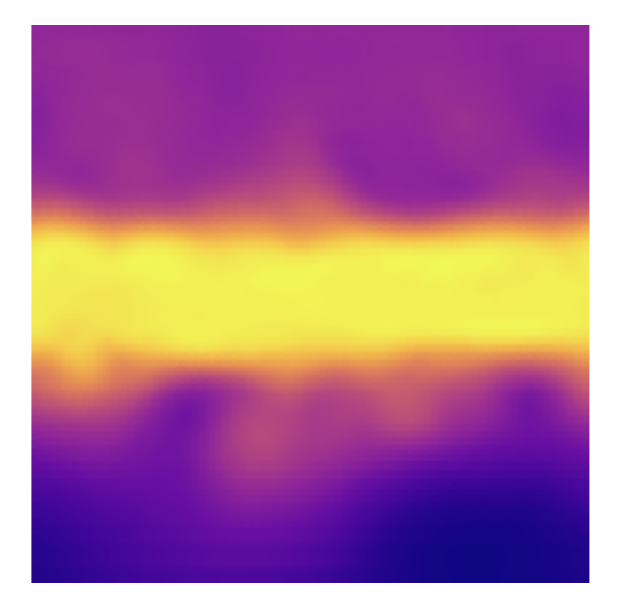
\includegraphics[width=0.9\linewidth]{figures/chapter-8/geopoth_mercator.png}
        \caption{ Geopotential height raster data as Mercator projected}
        \label{fig:merc_geopoth_raster}
    \end{minipage}\hfill
    \begin{minipage}{0.30\textwidth}
        \centering
        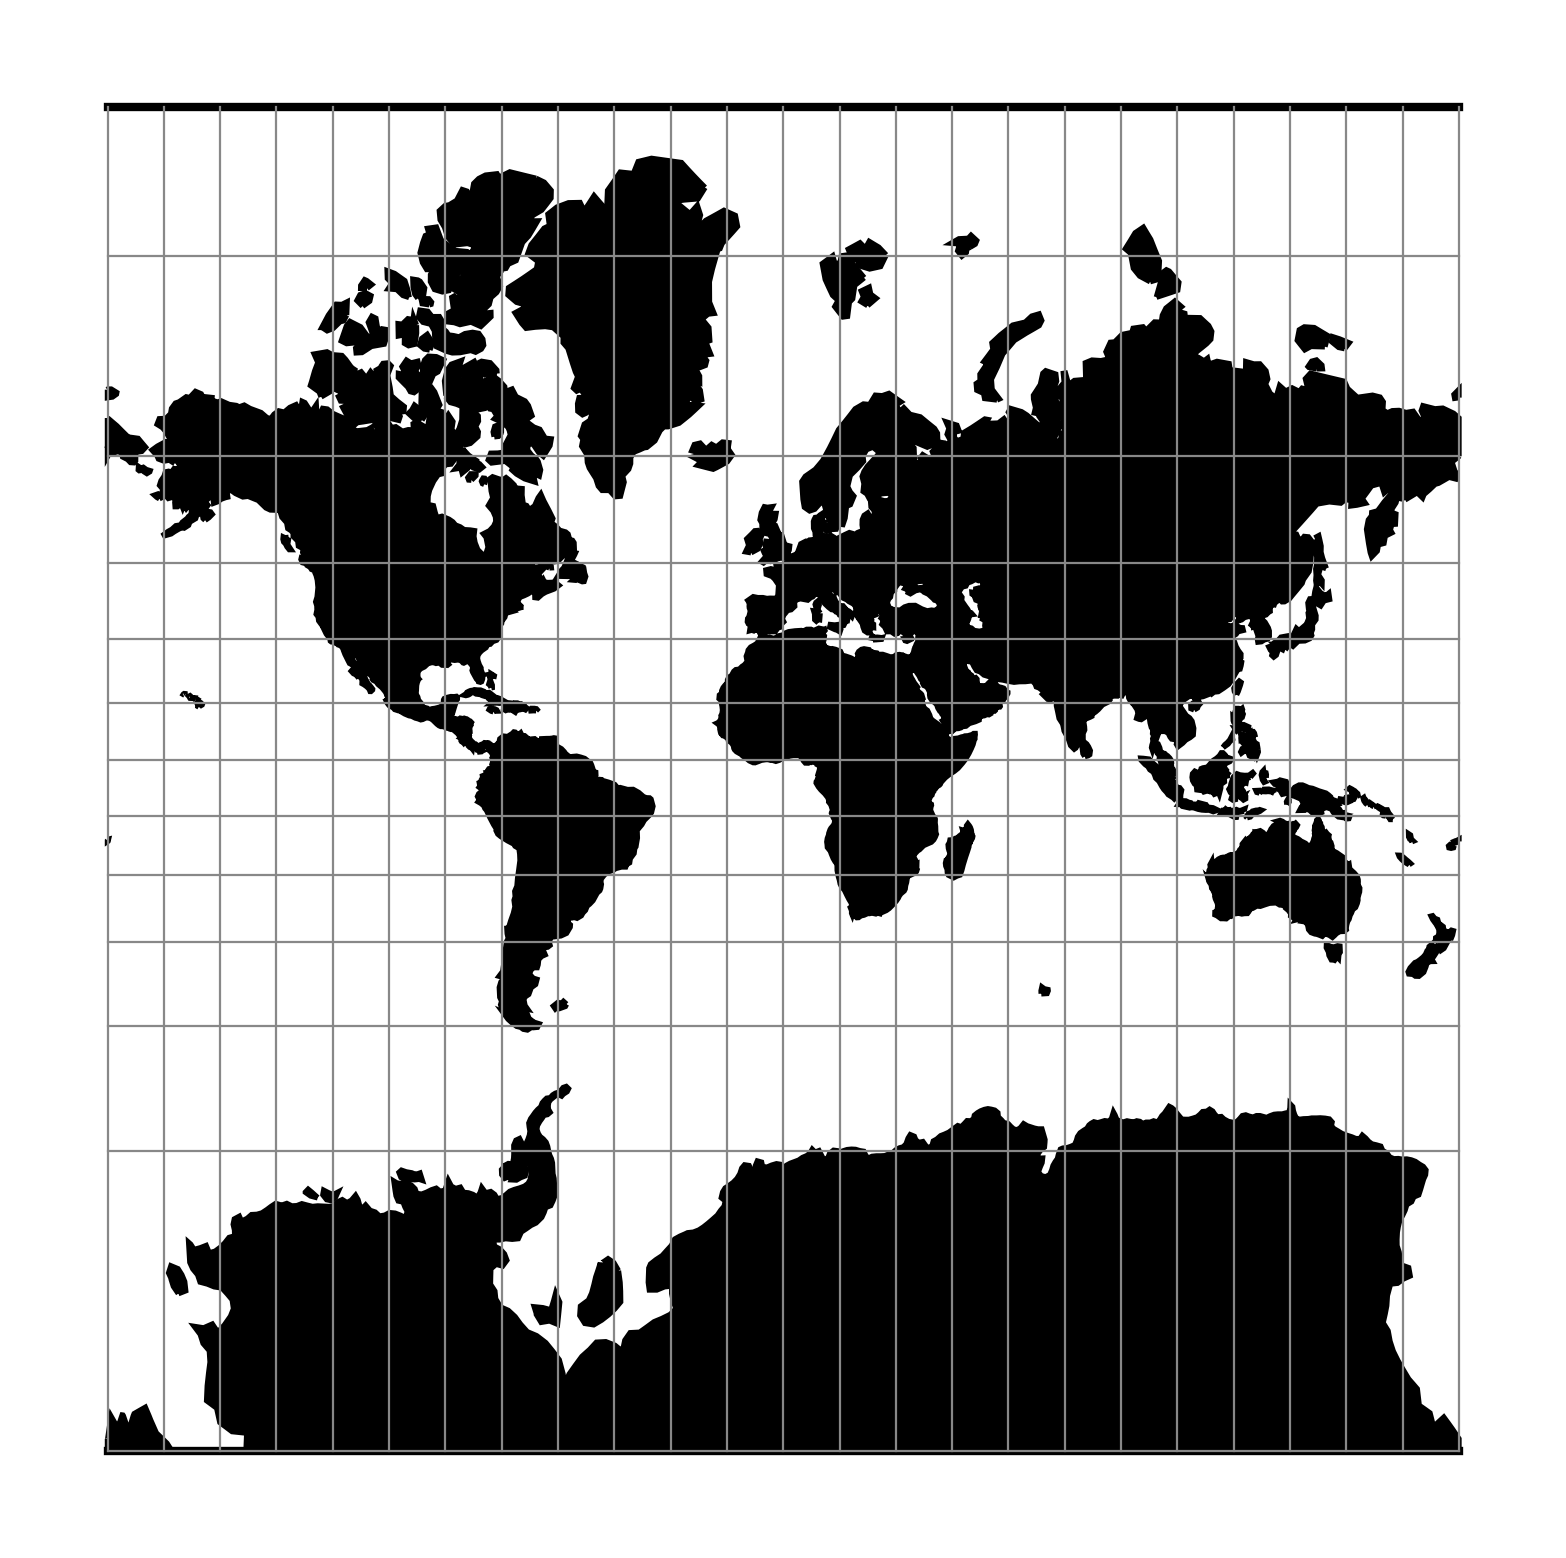
\includegraphics[width=0.9\linewidth]{figures/chapter-8/merc.png}
        \caption{Mercator Projection (Source \cite{PROJ_SITE})}
        \label{fig:merc_proj}
    \end{minipage}\hfill
    \begin{minipage}{0.30\textwidth}
        \centering
        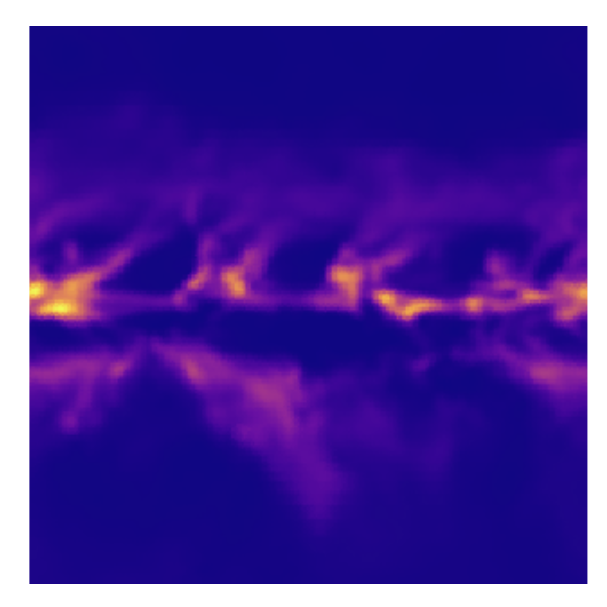
\includegraphics[width=0.9\linewidth]{figures/chapter-8/prect_mercator.png}
        \caption{Precipitation raster data as Mercator projected}
        \label{fig:merc_prect_raster}
    \end{minipage}\hfill
\end{figure}

\begin{figure}[H]
    \centering
    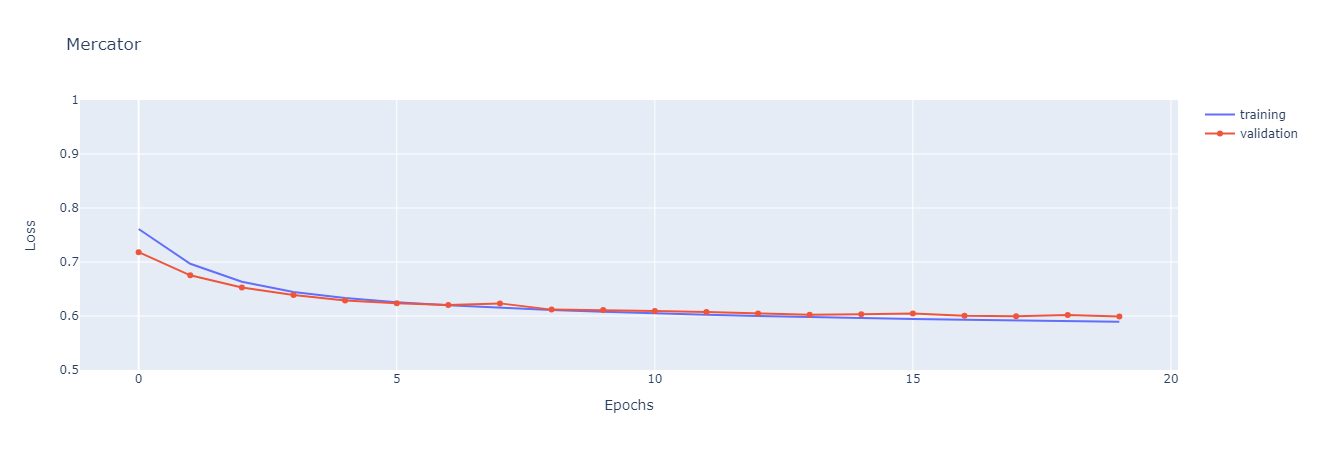
\includegraphics[width=1.0\linewidth]{figures/chapter-8/merc_loss.png}
    \caption{Mercator: Averaged training loss of models  }
    \label{fig:merc_loss}
\end{figure}

\newpage

\subsection{Plate Carree}

\begin{figure}[H]
    \centering
    \begin{minipage}{0.30\textwidth}
        \centering
        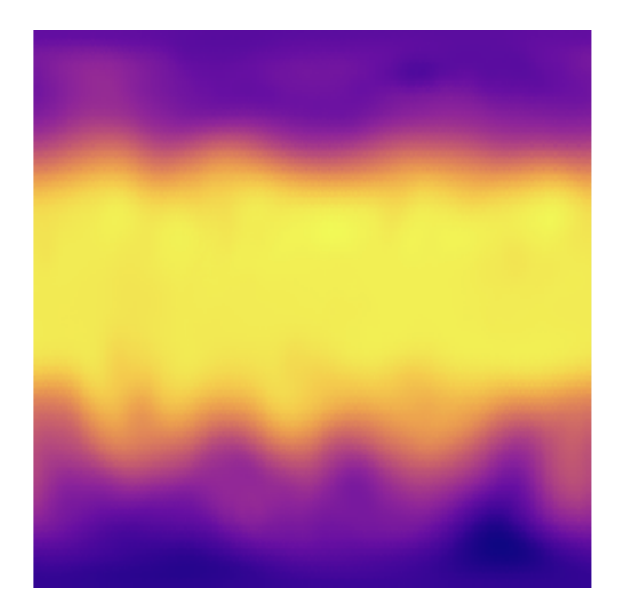
\includegraphics[width=0.9\linewidth]{figures/chapter-8/plate_caree_geopoth_raster.png}
        \caption{ Geopotential height raster data as Plate Carree projected}
        \label{fig:eqc_geopoth_raster}
    \end{minipage}\hfill
    \begin{minipage}{0.30\textwidth}
        \centering
        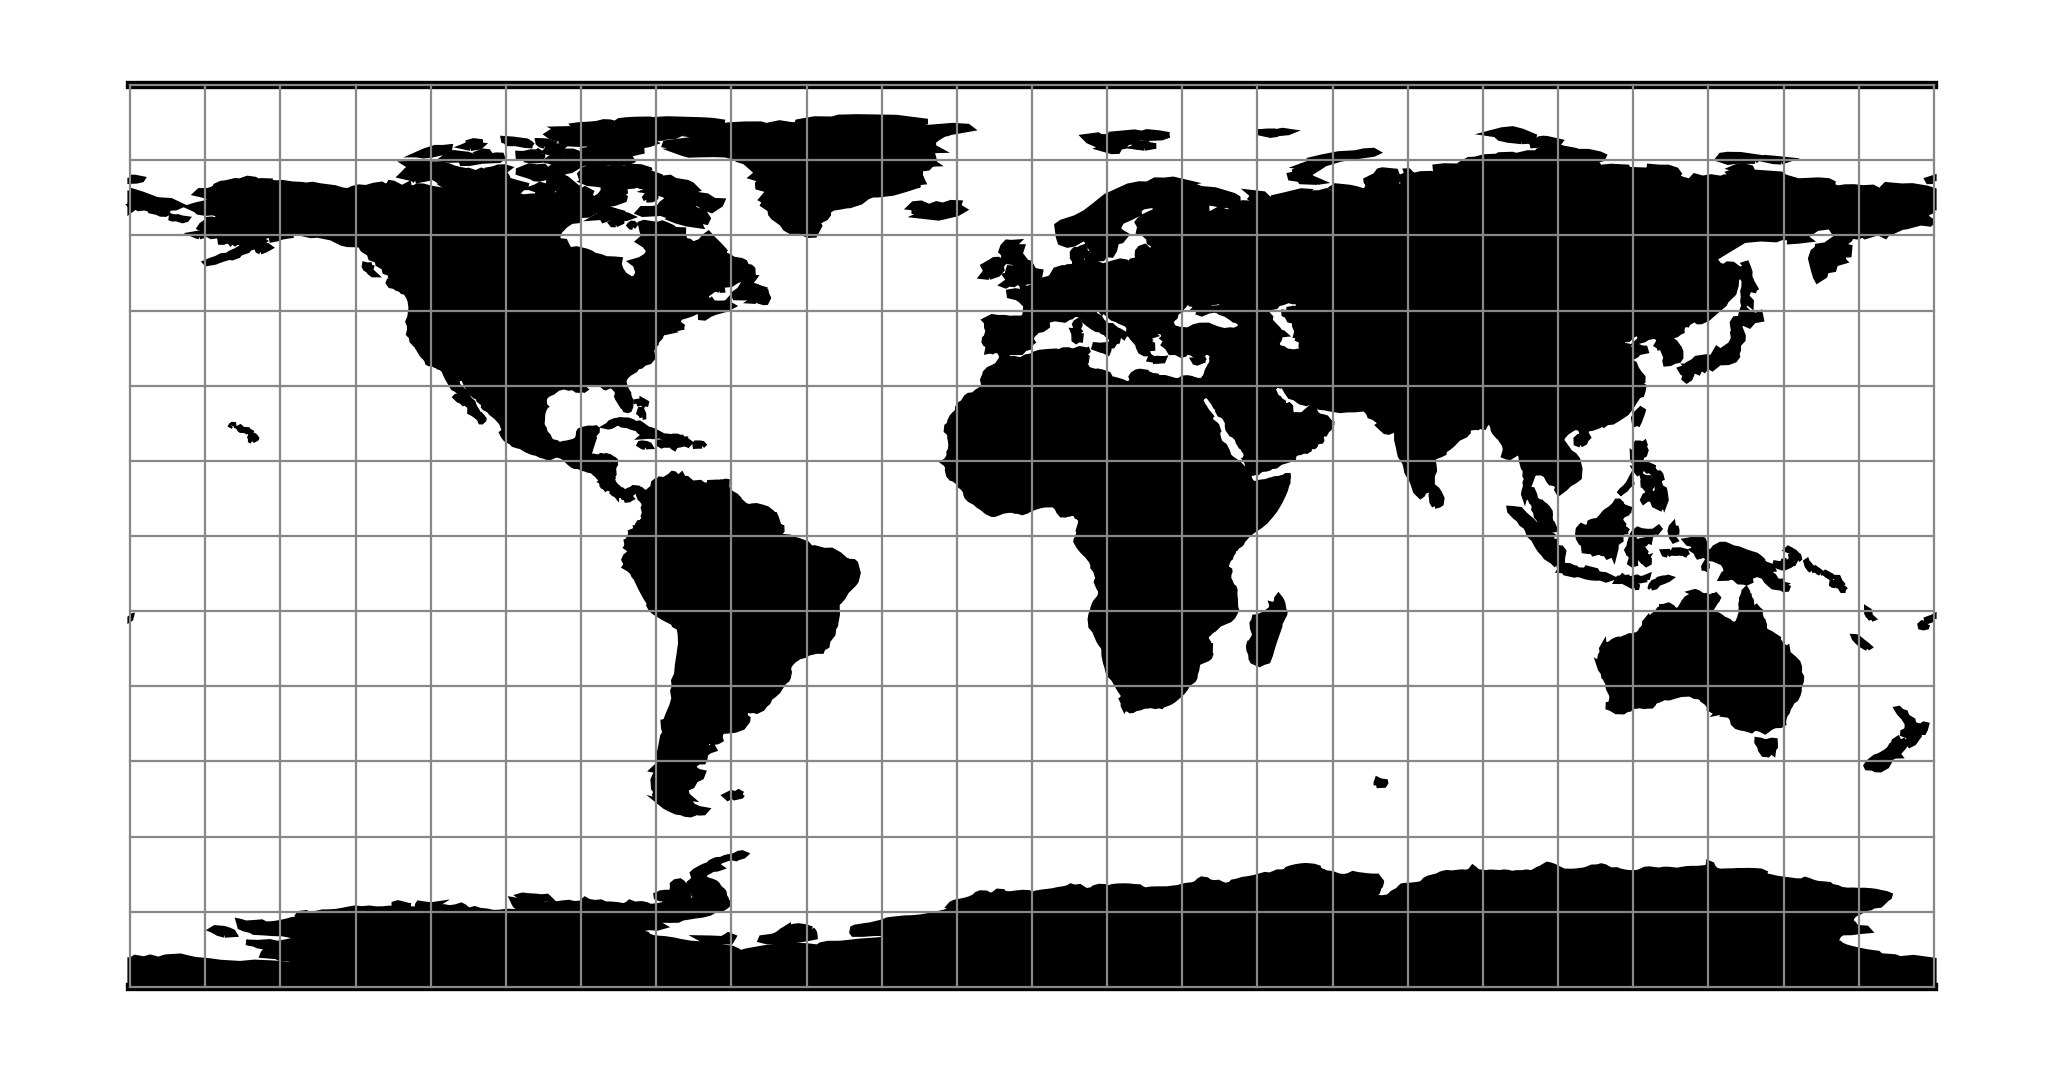
\includegraphics[width=0.9\linewidth]{figures/chapter-8/eqc.png}
        \caption{Plate Carree Projection (Source \cite{PROJ_SITE})}
        \label{fig:eqc_prect_raster}
    \end{minipage}\hfill
    \begin{minipage}{0.30\textwidth}
        \centering
        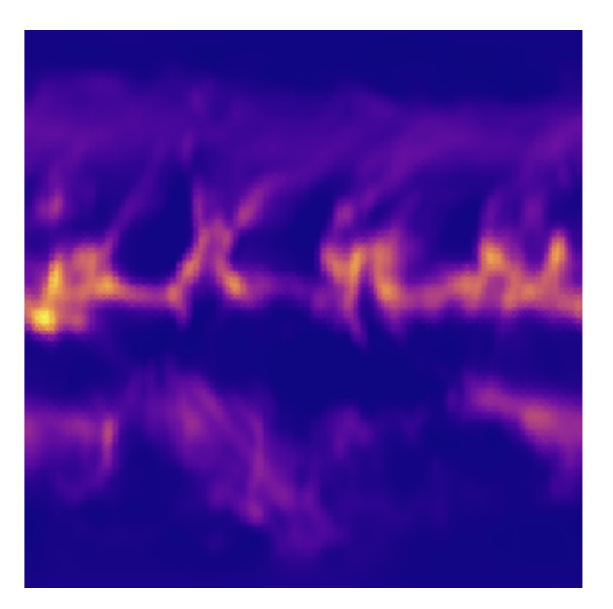
\includegraphics[width=0.9\linewidth]{figures/chapter-8/plate_caree_prect_raster.png}
        \caption{Precipitation raster data as Plate Carree projected}
        \label{fig:eqc_prect_raster}
    \end{minipage}\hfill
\end{figure}

\begin{figure}[H]
    \centering
    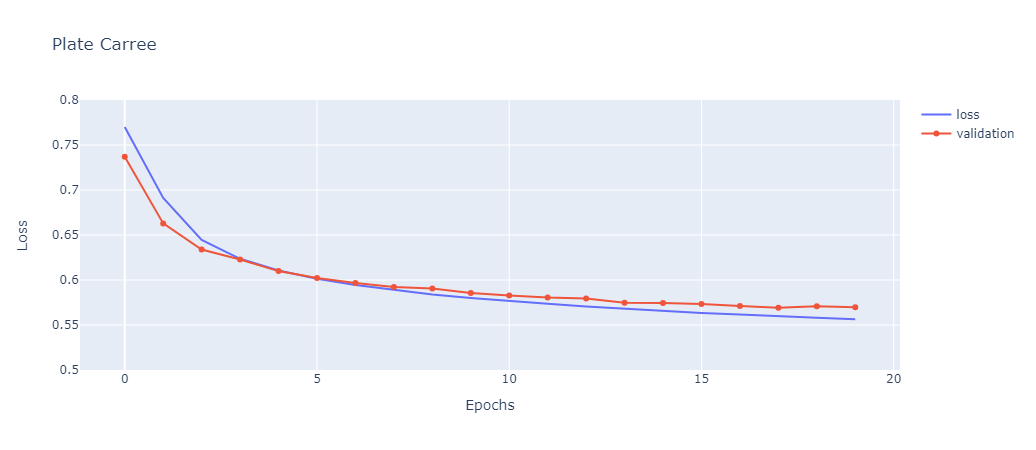
\includegraphics[width=1.0\linewidth]{figures/chapter-8/pc_loss.png}
    \caption{Plate Carree: Averaged training loss of models  }
    \label{fig:pc_loss}
\end{figure}

The trend for the training of the model


\subsection{Cylindrical Equal Area}

\begin{figure}[H]
    \centering
    \begin{minipage}{0.30\textwidth}
        \centering
        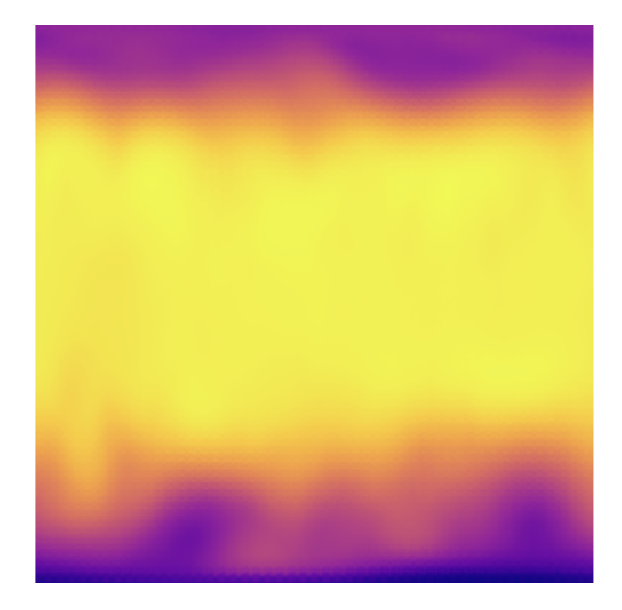
\includegraphics[width=0.9\linewidth]{figures/chapter-8/prect_cea.png}
        \caption{ Geopotential height raster data as Cylindrical Equal Area projected}
        \label{fig:cea_geopoth_raster}
    \end{minipage}\hfill
    \begin{minipage}{0.30\textwidth}
        \centering
        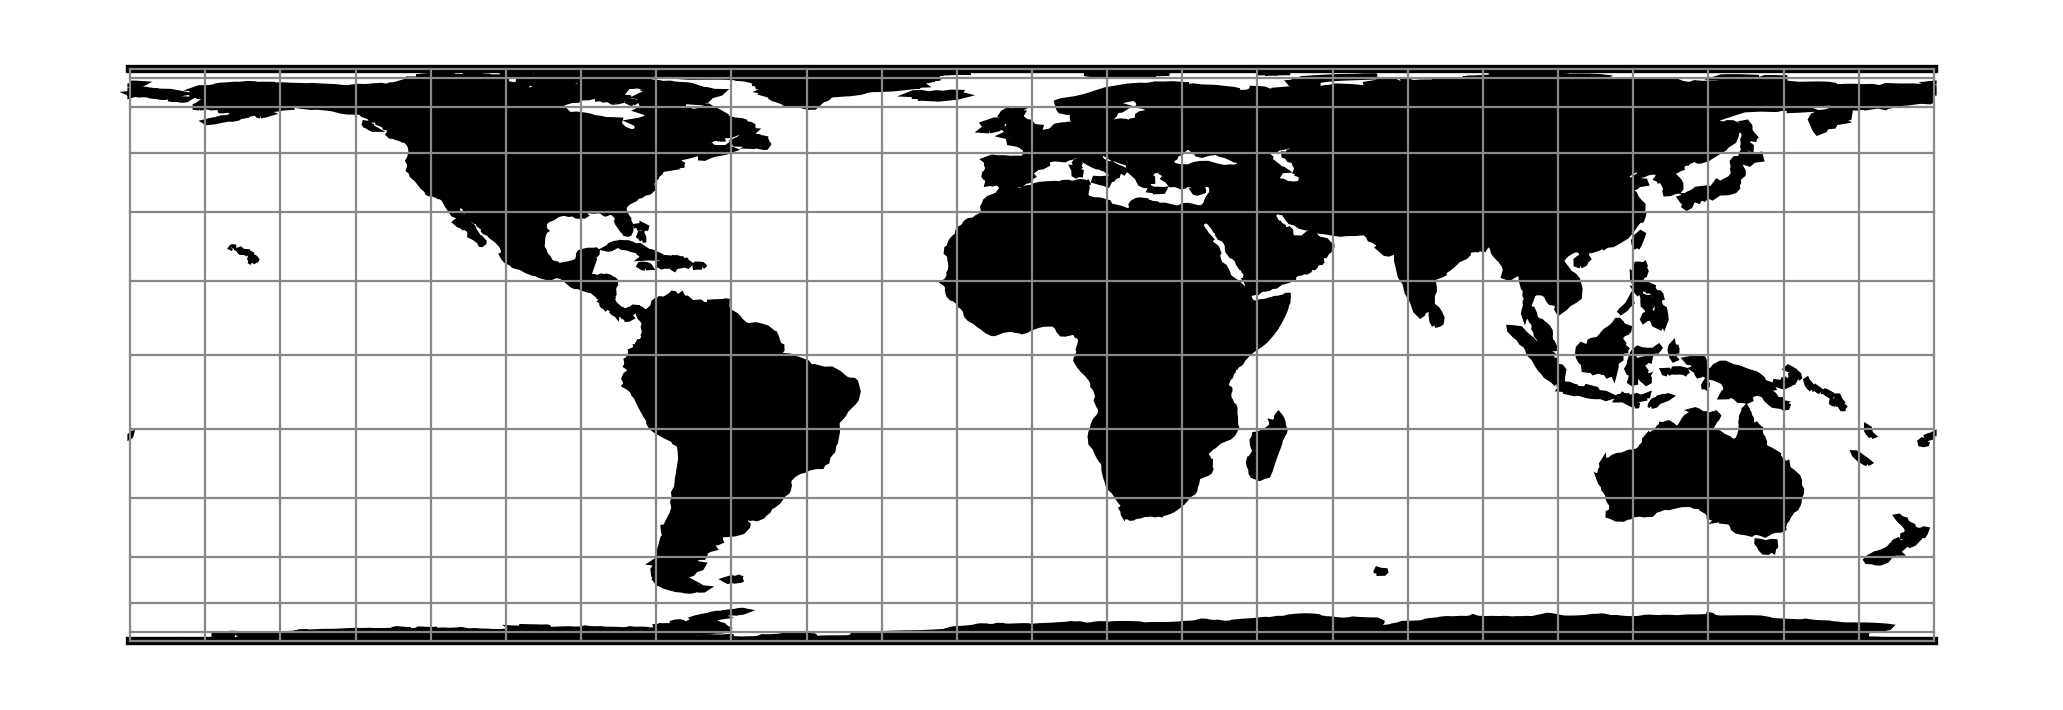
\includegraphics[width=0.9\linewidth]{figures/chapter-8/cea.png}
        \caption{Cylindrical Equal Area Projection (Source \cite{PROJ_SITE})}
        \label{fig:cea_prect_raster}
    \end{minipage}\hfill
    \begin{minipage}{0.30\textwidth}
        \centering
        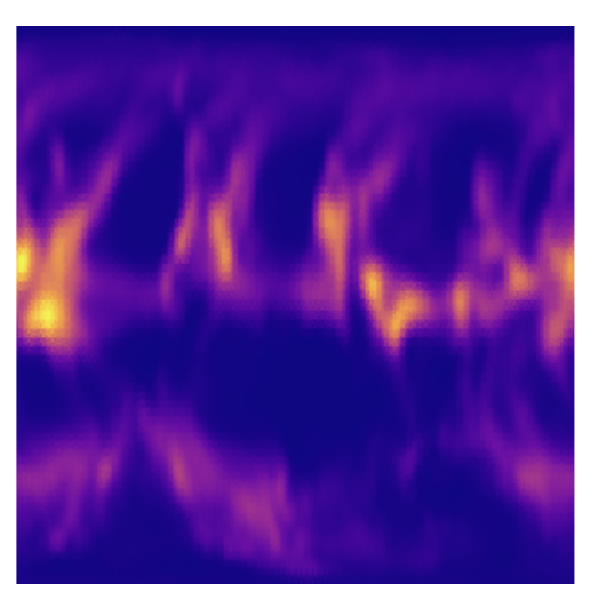
\includegraphics[width=0.9\linewidth]{figures/chapter-8/geopoth_cea.png}
        \caption{Precipitation raster data as Cylindrical Equal Area projected}
        \label{fig:cea_prect_raster}
    \end{minipage}\hfill
\end{figure}

\begin{figure}[h]
    \centering
    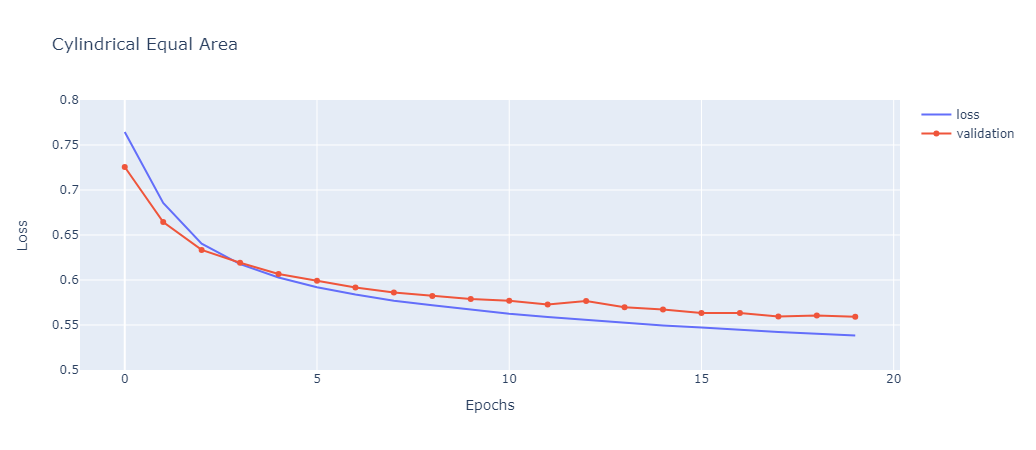
\includegraphics[width=1.0\linewidth]{figures/chapter-8/cea_loss.png}
    \caption{Cylindrical Equal Area: Averaged training loss of models  }
    \label{fig:cea_loss}
\end{figure}

\subsection{General Oblique Transformation}
\begin{figure}[H]
    \centering
    \begin{minipage}{0.30\textwidth}
        \centering
        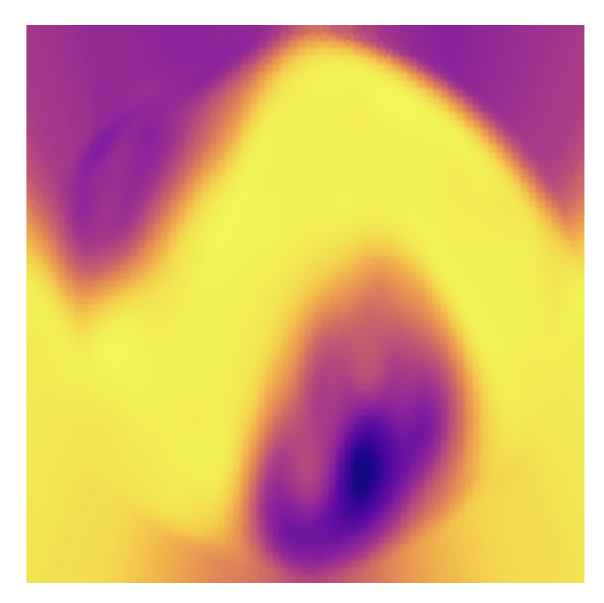
\includegraphics[width=0.9\linewidth]{figures/chapter-8/geopoth_got.png}
        \caption{ Geopotential height raster data as General Oblique Transformation projected}
        \label{fig:ob_tran_geopoth_raster}
    \end{minipage}\hfill
    \begin{minipage}{0.30\textwidth}
        \centering
        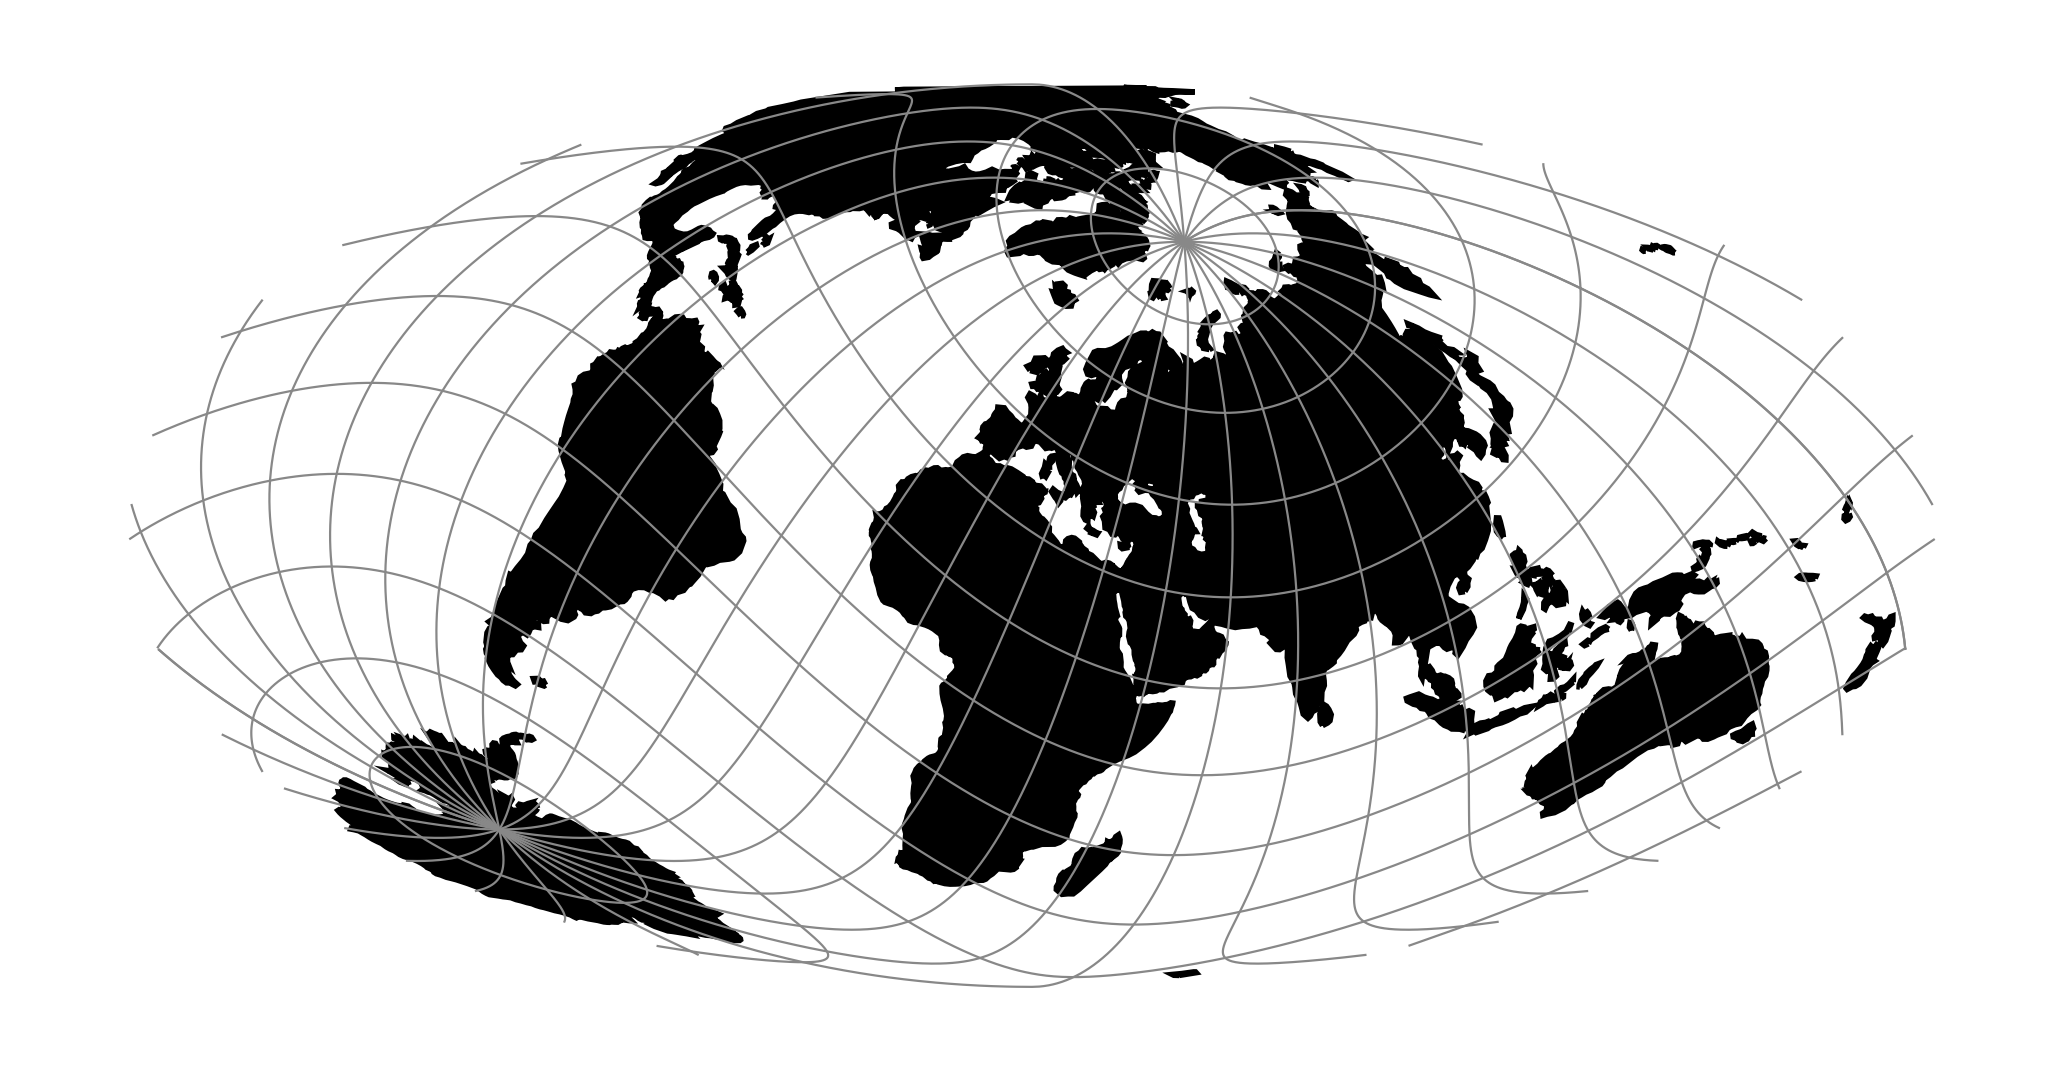
\includegraphics[width=0.9\linewidth]{figures/chapter-8/ob_tran.png}
        \caption{General Oblique Transformation Projection (Source \cite{PROJ_SITE})}
        \label{fig:ob_tran_proj}
    \end{minipage}\hfill
    \begin{minipage}{0.30\textwidth}
        \centering
        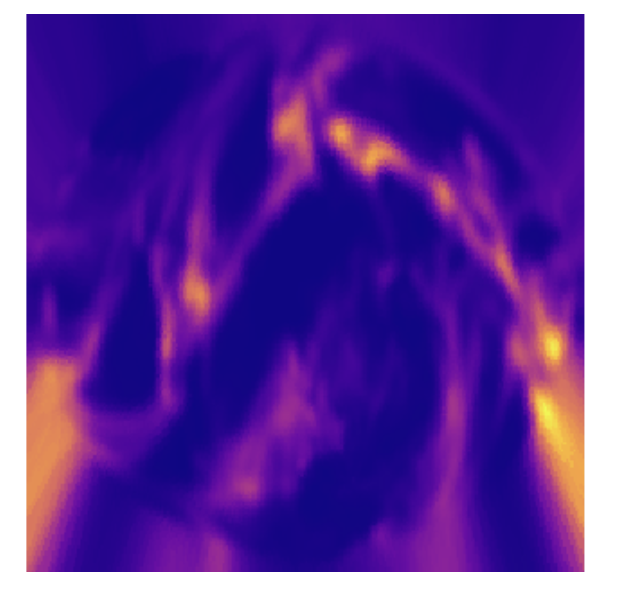
\includegraphics[width=0.9\linewidth]{figures/chapter-8/prect_got.png}
        \caption{Precipitation raster data as General Oblique Transformation projected}
        \label{fig:ob_tran_prect_raster}
    \end{minipage}\hfill
\end{figure}

\begin{figure}[H]
    \centering
    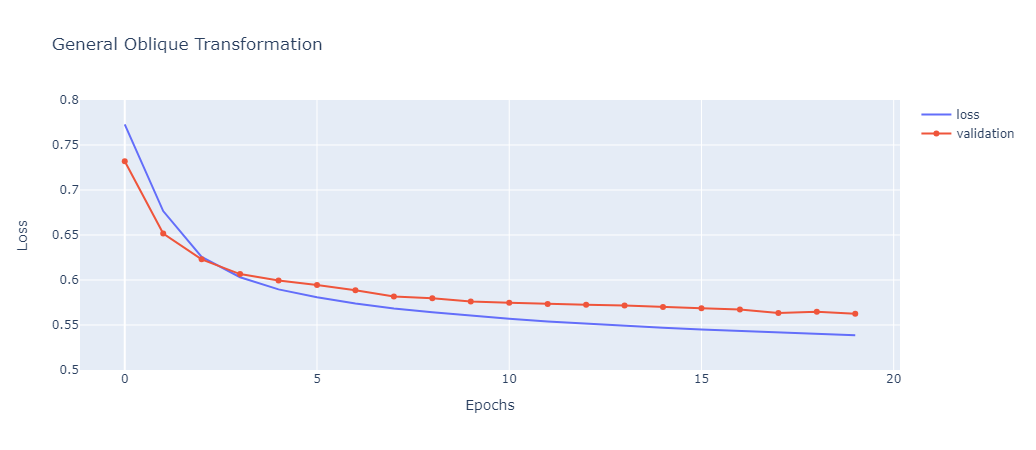
\includegraphics[width=1.0\linewidth]{figures/chapter-8/got_loss.png}
    \caption{General Oblique Transformation: Averaged training loss of models  }
    \label{fig:got_loss}
\end{figure}
\subsection{Results \& Observations}
\begin{itemize}
    \item The Figure~\ref{fig:merc_loss} shows the average training loss for the U-Net model mentioned in the \autoref{chap:approach}, it could be seen that model's training loss is stabilizing and the trend of the validation loss is on a decrease.
          The model is being trained well for the Mercator projection, we need to consider the fact that we have trained a shallow model with less numbers of filters.
    \item The Figure~\ref{fig:pc_loss} shows the average training loss decreasing and the trend of the validation loss is on an increase after the 17th epoch, with more training the model is on the path to overfit. Early stopping should have been used earlier for this projection dataset.
    \item Figure~\ref{fig:cea_loss} depicts that the model in training is subjected to overfit very quickly in the training process. Just after the 7th epoch the model is overfitting.
    \item Figure~\ref{fig:got_loss} shows, the model start to overfit from the 5th epoch.
    \item As soon as the rasters which are generated to resolve some of the distortions occurring due to map projections the rasters.
          The cylindrical equal area projection does resolve the distortion of area but is not able to perform well during the training of the model under observation.
          Same is the case with oblique general transformation projection, as it brings the north polar region at the central level part, but brings huge distortions equator regions.
    \item In our case the input data to the model, geopotential height when subjected to the whole raster, the model in under consideration tends to overfit.
    \item The Table~\ref{cylindrical_results_table} depicts the MAE to measure the quality of the predictions of the precipitation on the average results.

\end{itemize}
\begin{table}[ht]
    \centering
    \caption{Summary of Cylindrical Projection Model Performance}
    \label{cylindrical_results_table}
    \renewcommand{\arraystretch}{1.2} % Adjusts the row height
    \begin{tabular}{|l|c|c|c|c|c|}
        \hline
        \rowcolor[gray]{0.9}
        \textbf{\emph{Projection}}     & \textbf{\emph{\# Epochs}} & \textbf{\emph{MAE}} & \textbf{\emph{Validation MAE}} \\ \hline
        Mercator                       & 20                        & 0.51                & 0.51                           \\ \hline
        Plate Carree                   & 20                        & 0.49                & 0.49                           \\ \hline
        Cylindrical Equal Area         & 20                        & 0.48                & 0.49                           \\ \hline
        General Oblique Transformation & 20                        & 0.48                & 0.49                           \\ \hline
    \end{tabular}


\end{table}